\documentclass{article}
% Chinese
% \documentclass[UTF8, nofonts, mathptmx, 12pt, onecolumn]{article}
% \usepackage{xeCJK}
% \setCJKmainfont{SimSun}
\usepackage{amsmath}
\usepackage{amsfonts}
\usepackage{amssymb}
\usepackage{wasysym}
% \usepackage{ctex}
\usepackage{graphicx}
\usepackage{float}
\usepackage{geometry}
\geometry{a4paper,scale=0.8}
\usepackage{caption}
\usepackage{subcaption}
\usepackage{color}
% \newcommand{\oiint}{\mathop{{\int\!\!\!\!\!\int}\mkern-21mu \bigcirc} {}}
\newcommand*{\dif}{\mathop{}\!\mathrm{d}}
\newcommand*{\md}{\mathop{}\!\mathrm{d}}
\newcommand*{\me}{\mathrm{e}}

% \usepackage{parskip}
% \setlength{\parindent}{0cm}

\usepackage{bm}
\let\Oldmathbf\mathbf
\renewcommand{\mathbf}[1]{\boldsymbol{\Oldmathbf{#1}}}
\let\eqnarray\align

\renewcommand*{\arraystretch}{2}
\usepackage{units}
\renewcommand{\frac}{\nicefrac}

\usepackage{cellspace}
\setlength{\cellspacetoplimit}{5pt}
\setlength{\cellspacebottomlimit}{5pt}


\author{Xiping Hu}
\usepackage{authblk}
\author{Xiping Hu}
\affil{https://hxp.plus/}
\title{Homework for Chapter 7}

\begin{document}
\maketitle

\begin{figure}[H]
  \centering
  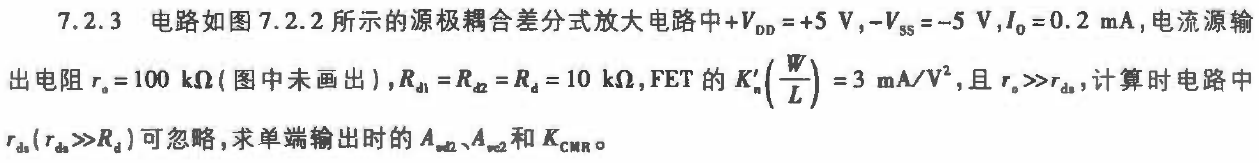
\includegraphics[width=\linewidth]{figures/Problem723} 
  \label{fig:}
\end{figure}

\begin{figure}[H]
  \centering
  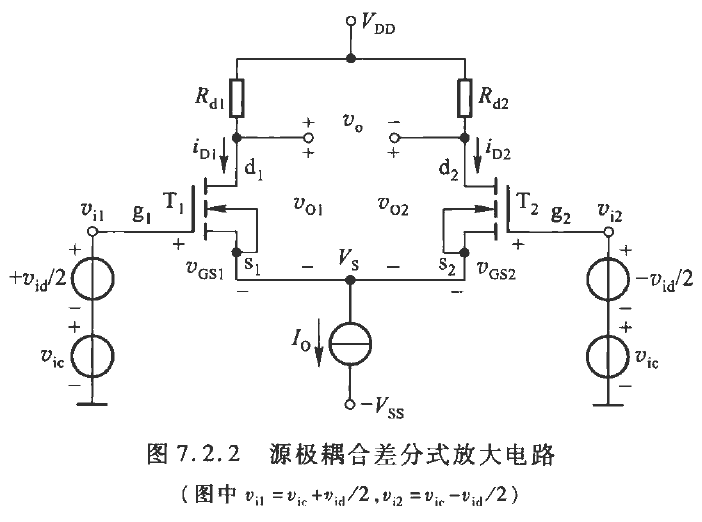
\includegraphics[width=0.7\linewidth]{figures/Problem7231} 
  \label{fig:}
\end{figure}

\begin{equation*}
  \begin{aligned}
    I_{D1} = \dfrac{I_0}{2} = K_n \left( V_{GS2} - V_{TN2} \right)^2 \Rightarrow V_{GS2} - V_{TN2} = \sqrt{\dfrac{\frac{I_0}{2} }{\frac{K_n}{2} } } = 0.26 \  \mathrm{V}
  \end{aligned}
\end{equation*}

\begin{equation*}
  \begin{aligned}
    g_m = 2 K_n \left( V_{GS2} - V_{TN2} \right) = 0.78 \  \mathrm{mS}
  \end{aligned}
\end{equation*}

\begin{equation*}
  \left\{
    \begin{aligned}
      & A_{vd2} = \dfrac{1}{2} g_m R_d = 3.9 \\
      & A_{vc2} = - \dfrac{R_d}{2 r_o} = - 0.05 \\
      & K_{CMR} = \left| \dfrac{A_{vd2}}{A_{vc2}}  \right| = 78
    \end{aligned}
  \right.
\end{equation*}




\end{document}